\section{Variedades Suaves}\label{Sección: Variedades Suaves}
Las variedades topológicas tienen propiedades muy interesantes en sí mismas, sin embargo, para nuestros fines lo que nos interesa es poder realizar cálculos en ellas, en particular darle sentido a la noción de diferenciabilidad. Esto no es posible en general, es con este fin que daremos algunas definiciones que nos permitirán construir una estructura adicional con la cual podremos dotar a algunas variedades topológicas; esta estructura será lo que nos permitirá dar sentido a la derivada.

Cuando decimos que una función $f$ es diferenciable o suave lo que queremos decir es que: Si $U$ y $V$ son subconjuntos abiertos de $\R^n$ y $\R^m$ respectivamente, entonces  $f: U \to V$ tiene derivadas parciales de todos los órdenes. Al conjunto de funciones con esta propiedad usualmente se le denota como $C^{\infty}$ y se dice que las funciones son de clase $C^{\infty}$.


\begin{definition}[Mapa de Transición]\label{Definición: Mapa de Transición}
	Sea $M^n$ una variedad topológica y $(U,\phi)$, $(V,\psi)$ cartas en $M$. Si $U \cap V \neq \varnothing$, entonces a la composición $\psi \circ \phi^{-1}: \phi(U \cap V) \to \psi(U \cap V)$ es llamada el \it{mapa de transición de $\phi$ a $\psi$}
\end{definition}

\begin{definition}[Cartas Suavemente Compatibles]\label{Definición: Cartas Suavemente Compatibles}
	Diremos que dos cartas $(U,\phi)$ y $(V,\psi)$ son \it{suavemente compatibles} o $C^{\infty}-$compatibles si $U \cap V = \varnothing$ o si los mapas de transición
	\[ \psi \circ \phi^{-1}: \phi(U \cap V) \to \psi(U \cap V), \quad \phi \circ \psi^{-1}: \psi(U \cap V) \to \phi(U \cap V) \]
	son ambos suaves.
\end{definition}

\begin{figure}[h]
	\centering
	\begin{tikzpicture}[scale=1]
	\coordinate (a) at (0,0);
	\path[draw,use Hobby shortcut,closed=true,thick]
	(0,2.5) .. (2,2.5) .. (1,4.5) .. (.3,4.5) .. (-1,4) .. (-2,2.5);

	\begin{scope}
		\clip (0.25,3.5) circle (0.5);
		\fill[blue!30!white,opacity=0.5] (-0.25,3.25) circle (0.5);
	\end{scope}
	\draw[dashed] (0.25,3.5) circle (0.5);
	\draw[dashed] (-0.25,3.25) circle (0.5);
	\draw node at (0.8,4) {$V$};
	\draw node at (-0.9,2.75) {$U$};

	\draw [thick, <->] (-5,0) -- (-1,0);
	\draw [thick, <->] (-3,-2) -- (-3,2);
	\draw [thick, <->] (1,0) -- (5,0);
	\draw [thick, <->] (3,-2) -- (3,2);

	\begin{scope}
		\clip (-3,0.5) ellipse  (0.8 and 1);
    \fill[color=blue!30!white,opacity=0.5] (-2.5,0) ellipse  (1.2 and 0.8);
	\end{scope}
	\draw [dashed,thick] (-3,0.5) ellipse  (0.8 and 1);
	% \draw [dashed,thick] (-2.5,0) ellipse  (1.2 and 0.8);

	\begin{scope}
		\clip (3,0.5) ellipse  (0.8 and 1);
		\fill[color=blue!30!white,opacity=0.5](3.5,0) ellipse  (1.2 and 0.8);
	\end{scope}
	% \draw [dashed,thick] (3,0.5) ellipse  (0.8 and 1);
	\draw [dashed,thick] (3.5,0) ellipse  (1.2 and 0.8);

	\draw[line width=1, ->] (1,3.75) arc (90:-5:2.5);
	\draw[line width=1, ->] (-1,3.25) arc (-90:0:-1.5);
	\draw[line width=1, ->] (-1.75,0.5) -- (2,0.5);

	\draw node at (-2.5,2.75) {$\phi$};
	\draw node at (3.25,3) {$\psi$};
	\draw node at (-4.25,1.25) {$\phi(U)$};
	\draw node at (4.5,1) {$\psi(V)$};
	\draw node at (0.25,1) {$\psi \circ \phi^{-1}$};


\end{tikzpicture}

	\caption{Mapa de Transición}
\end{figure}

Verificar que dos cartas son suavemente compatibles es relativamente sencillo, dado que el mapa de transición es una composición de homeomorfismos este será un homeomorfismo, así, únicamente habrá que verificar que la función y su inversa son diferenciables.

\begin{definition}[Atlas, Atlas Suave y Atlas Maximal]\label{Definición: Atlas}
	Sea $M$ una variedad topológica. Un \it{atlas} en $M$, denotado como $\A$, es una colección indexada $\{(U_i,\phi_i)\}_{i\in I}$ de cartas en $M$ que cubren a la variedad, esto es:
	\[\bigcup_{i \in I} U_i = M. \]

	Si cualesquiera dos cartas en un atlas son suavemente compatibles, entonces diremos que el atlas es un \it{atlas suave}. A las cartas que forman a un atlas suave se les llama \it{cartas suaves}.

	Un atlas $\A$ estará contenido en otro atlas $\mathcal{B}$ si cada carta $(U,\phi)$ que pertenece a $\A$ también pertenece a $\mathcal{B}$. Diremos que un atlas suave $\A$ es \it{maximal} si no está propiamente contenido en ningún atlas más grande.
\end{definition}

\begin{definition}[Variedad Suave]\label{Definición: Variedad Suave}
	Sea $M$ una variedad topológica. Una \it{variedad suave} será un par $(M, \A)$, donde $\A$ es un atlas maximal en $M$. Usualmente a $\A$ se le llama la \it{estructura suave} en $M$.
\end{definition}

Por conveniencia, en lugar de escribir \enquote{Sea $(M,\A)$ una variedad suave} diremos simplemente \enquote{Sea $M$ una variedad suave}; esto cuando la estructura suave se pueda entender a partir del contexto o no sea necesario referirnos a ella de forma explícita.


Si quisiéramos definir una función $f: M \to \R$ como suave, quizá pudiésemos haber estado inclinados a dar la siguiente definición: \enquote{Una función $f: M \to \R$ es diferenciable si y sólo si para cada carta $(U,\phi)$ se tiene que $f\circ \phi^{-1}: \phi(U) \to \R$ es una función diferenciable}, esta definición podría parecernos más natural, sin embargo, presenta un problema de ambigüedad ya que, para una misma variedad pueden existir muchos atlas diferentes y estos pueden generar la misma estructura o estructuras similares pero distintas, como veremos en los siguientes ejemplos.
\begin{figure}[h]
	\begin{center}
		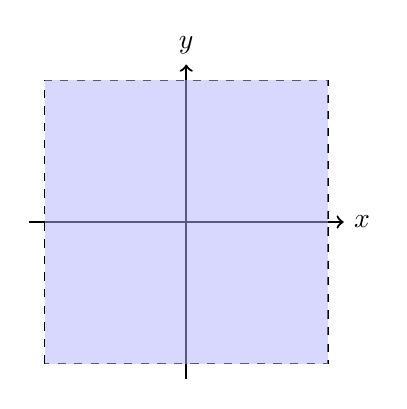
\begin{tikzpicture}[scale=2, baseline={(0,-1.5)}]
\draw[color=black,thick,->] (-1,0) -- (1,0) node[anchor=west]{$x$};%
\draw[color=black,thick,->] (0,-1) -- (0,1) node[anchor=south]{$y$};%

\draw[dashed] (-0.90,-0.90) rectangle (0.90,0.90);
\path[fill=blue!30!white,opacity=0.5] (-0.90,-0.90) rectangle (0.90,0.90);

\end{tikzpicture}

		\caption{Representación de $\R^2$ siendo cubierta por una única carta.}
	\end{center}
\end{figure}

\begin{example}[Variedades Cubiertas Por Una Única Carta]\label{Ex: Variedad Suave - Carta Unica}
	Si $M^n$ es una variedad topológica y existe un atlas para $M$ que contiene a una única carta entonces la carta define una estructura suave para la variedad, esto dado que trivialmente cumplirá el ser suavemente compatible con cualquier otra carta en el atlas.
\end{example}


\begin{example}[Espacios Euclidianos]\label{Ex: Variedad Suave - Espacios Euclidianos}
	Si tomamos cualquier espacio Euclidiano $\R^n$ podemos dar el atlas formado únicamente por la carta $(\R^n,\id_{\R^n})$, por el ejemplo anterior sabemos que esta carta define una estructura suave en $\R^n$.
\end{example}

\begin{example} % Ejemplo de diferentes estructuras suaves.
	Podemos considerar la función $\psi: \R \to \R$, definida del siguiente modo:
	\[
		\psi(x) = x^3
	\]

	Esta función es un homeomorfismo, y por los ejemplos anteriores sabemos que $(\R, \psi(x))$ es una variedad suave, con la estructura definida por  $\psi$. Sin embargo, al considerar el mapa de transición tenemos que $\id_{\R} \circ \psi^{-1}(y) = y^{\frac{1}{3}}$, y esta función no es diferenciable en el origen, por lo cual las cartas no son suavemente compatibles, y las estructuras determinadas por $(\R, \id_{\R})$ y $(\R,\psi)$ serán diferentes.
\end{example}

Para resolver este problema de ambigüedad es que hemos introducido el concepto atlas maximal. Lo que el atlas maximal nos garantiza es que cada carta que sea suavemente compatible con cualquier otra carta en el atlas estará ya incluida en el mismo.

\begin{theorem}
	Si $M$ es una variedad topológica, entonces cada atlas suave $\A$ de $M$ está contenido en un atlas suave maximal único, llamado la \it{estructura suave determinada por $\A$}.
\end{theorem}

\begin{proof}
	Sea $\A$ un atlas suave para $M$ y sea $\bar{\A}$ el conjunto de todas las cartas que son suavemente compatibles con todas las cartas de $\A$.
	\begin{enumerate}
		\item $\bar{A}$ es un atlas suave. Consideremos dos cartas arbitrarias $(U,\phi)$ y $(V,\psi)$ en $\bar{\A}$, además consideremos un punto arbitrario $\phi(p) \in \phi(U \cap V)$. Por definición el atlas $\A$ cubre a $M$, por lo que existirá una carta $(W,\theta)$ en $\bar{A}$ tal que $p \in W$, por construcción de $\bar{A}$ sabemos que $\psi \circ \theta^{-1}$ y $\theta \circ \phi^{-1}$ son suaves. Y, dado que $p \in U \cap V \cap W$, se sigue que $\psi \circ \phi^{-1} = (\psi \circ \theta^{-1}) \circ \theta \circ \phi^{-1}$, al ser una composición de funciones suaves será suave en $\phi(U \cap V)$, dado que hemos elegido las cartas $(U,\phi)$ y $(V,\psi)$ de manera arbitraria podemos concluir que $\bar{\A}$ es un atlas suave.
		\item $\bar{\A}$ es un atlas maximal. Si consideramos una carta que sea suavemente compatible con cualquier otra carta en $\bar{\A}$ por construcción esta carta deberá ser suavemente compatible con cualquier otra carta en $\A$, pero esto implica que la carta pertenece a $\bar{\A}$, por lo tanto $\bar{\A}$ es maximal.
		\item $\bar{\A}$ es único. Tomando algún otro atlas suave maximal $\mathcal{B}$ que contenga a $\A$ tendremos que cada una de sus cartas es suavemente compatible con cada carta en $\A$ por lo que $\mathcal{B} \subseteq \bar{\A}$, pero al ser $\mathcal{B}$ maximal se tendrá que $\mathcal{B} = \bar{A}$
	\end{enumerate}
\end{proof}

\begin{theorem}\label{Teorema: Unicidad de Estructura Suave}
	Dos atlas suaves para una variedad $M$ determinan la misma estructura suave si y sólo si su unión es un atlas suave.
\end{theorem}

\begin{proof}
	Sean $\A$ y $\mathcal{B}$ dos atlas suaves en $M$ y que ambos determinan la misma estructura suave. Por el teorema anterior sabemos que esto significa que existe un atlas suave maximal $\mathcal{C}$ tal que $\A \subset \mathcal{C}$ y $\mathcal{B} \subset \mathcal{C}$.

	Si consideramos una carta $(U,\phi) \in \A \cup \mathcal{B}$ esta deberá estar contenida en $\A$ o $\mathcal{B}$, podemos suponer sin pérdida de generalidad que está contenida en $\A$, también estará contenida en $\mathcal{C}$ y por construcción cada carta en $\mathcal{C}$ debe ser suavemente compatible con cada carta en $\mathcal{B}$, análogamente para el caso en que la carta está contenida en $\mathcal{B}$. Por lo tanto, podemos concluir que $\A \cup \mathcal{B}$ es un atlas suave.

	Supongamos ahora que $\A \cup \mathcal{B}$ es un atlas suave. Dado que las estructuras suaves determinadas por $\A$ y $\mathcal{B}$ ambas contendrán a $\A \cup \mathcal{B}$, y que por el teorema anterior hay una única estructura suave que contiene a $\A \cup \mathcal{B}$ podemos concluir que $\A$ y $\mathcal{B}$ determinan la misma estructura suave.
\end{proof}

Lo que estos dos teoremas nos permiten hacer es definir de manera más sencilla la estructura suave para una variedad, ya que, en lugar de tener que describir un atlas maximal podemos simplemente escoger algún atlas suave y sabemos que la estructura determinada será única.

Hay muchos ejemplos de variedad suaves y, como veremos a continuación, a cada una de las variedades topológicas que dimos como ejemplo anteriormente se le puede dar una estructura suave, sin embargo, esto no es cierto en general, hay ejemplos de variedades topológicas a las cuales no se les puede dar una estructura suave. Un resultado interesante que no veremos aquí es que, si $M^n$ es una variedad topológica con $n=1,2,3$, entonces a esta se le puede dar una estructura suave, esto fue probado por James Munkres en 1960, la demostración puede ser consultada en \enquote{\textcite{munkres1960obstructions}}.


\begin{example}[Espacios Vectoriales Finito-Dimensionales]\label{Ex: Variedad Sauve - Espacios Vectoriales}
  Sea $V$ un espacio vectorial finito dimensional. Sabemos que todo espacio vectorial tiene una base, esto como consecuencia del axioma de elección. Además, es posible hacer de cada espacio vectorial un espacio normado, y en el caso finito dimensional todas las normas en el espacio son equivalentes.

  Digamos que $\{x_1, \ldots, x_n\}$ es una base para $V$ y que $\| \cdot \|: V \to \R$ es una norma en $V$, cada norma determina una topología en $V$, y para cada base podemos definir un isomorfismo lineal canónico $\phi: V \to \R^n$, este isomorfismo esta dado como:
  \[
    \phi\left( \sum_{i=1}^{n} a_i x_i\right) = (a_1, \ldots, a_n)
  \]
  Con respecto a la topología inducida por la norma y por la linealidad de $\phi$ podemos garantizar que $\phi$ es continua, y por el mismo argumento, que su inversa $\phi^{-1}$ también lo es. Podemos concluir que $\phi$ es un homeomorfismo entre $V$ y $\R^n$, por lo cual, $V$ con la topología inducida por la norma será una variedad topológica.

  La estructura suave está determinada por la carta única $(V, \phi)$ que cubre a todo el espacio vectorial, por lo tanto, todo espacio vectorial finito dimensional es una variedad suave.
\end{example}

\begin{example}[Subconjuntos Abiertos De Variedades Suaves]\label{Ex: Variedad Suave - Subvariedades Suaves}
	Sea $M^n$ una variedad suave y $U$ un subconjunto abierto de $M$, entonces $U$ es una variedad suave.

	De modo similar al ejemplo \ref{Ex: Variedad Topologica - Bolas Abiertas} podemos mostrar que en general los subconjuntos abiertos de las variedades topológicas son, en sí mismos, variedades topológicas.

	Si $M$ es una variedad topológica y $U \subset M$ es abierto, entonces la topología inducida en $U$ heredará el ser Hausdorff y segundo numerable. Cada punto en $U$ está contenido en una carta de la variedad; dicha carta restringida a $U$ y el mapa coordenado nos da un homeomorfismo entre $U$ y algún conjunto abierto en $\R^n$, por lo que $U$ es una variedad topológica. Usualmente cuando hablamos de un subconjunto abierto de una variedad para enfatizar nos referiremos a él como una \it{subvariedad abierta}.

	Dado que $M$ es una variedad suave, existirá un atlas maximal $\A = \{(V_i,\phi_i) \}_{i \in I}$ en $M$, para cualquier conjunto abierto $U$ de $M$ podemos considerar el atlas:
	\[ \A_U = \{(V_i \cap U, \phi_i |_{V_i \cap U})\}_{i \in I} \]

	Como cada una de las cartas en $\A$ es suavemente compatible con cualquier otra carta en $\A$, sus restricciones a $V_i \cap U$ también serán suavemente compatible con cualquier otra carta en $\A$, en particular con aquellas restringidas a $V_i \cap U$. Por lo tanto $(U, \A_U)$ será una variedad suave.
\end{example}

\begin{example}[$n-$Esfera]
	La $n$-esfera $\S^n$ es una variedad suave.

	\begin{figure}[h]
		\begin{center}
			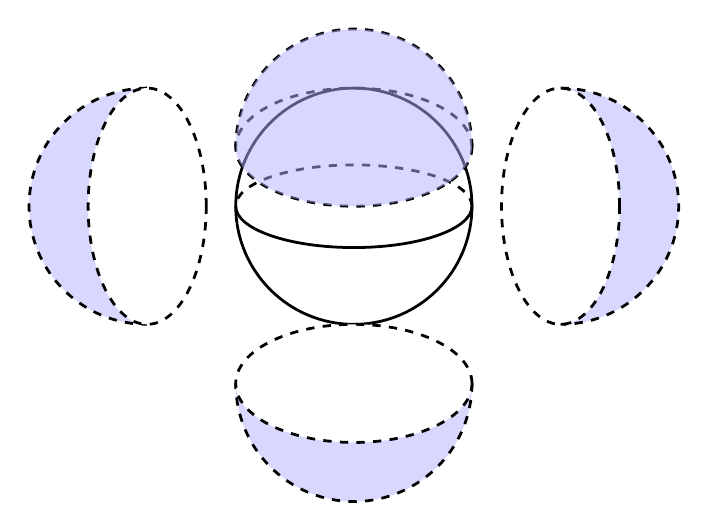
\begin{tikzpicture}[scale=1.5]
  \draw[line width=1, dashed] (1,0) arc (0:180:1 and 0.35);
  \draw[line width=1] (1,0) arc (0:180:1 and -0.35);
  \draw[line width=1](0,0) circle (1);

  % Left Chart
  \path[fill=blue!30!white,opacity=0.5] (-1.75,1) arc (90:-90:-1 and 1);
  \draw[line width=1, dashed] (-1.75,1) arc (90:-90:-1 and 1);
  \draw[fill=white, line width=1, dashed] (-1.75,0) ellipse (0.5 and 1);

  % Right Chart
  \path[fill=blue!30!white,opacity=0.5,line width=1, dashed] (1.75,1) arc (90:-90:1 and 1);
  \draw[fill=white, line width=1, dashed] (1.75,0) ellipse (0.5 and 1);
  \draw[line width=1, dashed] (1.75,1) arc (90:-90:1 and 1);

  % Top Chart
  \draw[line width=1, dashed] (0,0.5) ellipse (1 and 0.5);
  \draw[line width=1, dashed] (1,0.5) arc (0:180:1 and 1);
  \path[fill=blue!30!white,opacity=0.5] (1,0.5) arc (0:-180:1 and 0.5);
  \path[fill=blue!30!white,opacity=0.5] (1,0.5) arc (0:180:1 and 1);


  % Bottom Chart
  \path[fill=blue!30!white,opacity=0.5,line width=1, dashed] (1,-1.5) arc (0:-180:1 and 1);
  \draw[line width=1, dashed] (1,-1.5) arc (0:-180:1 and 1);
  \draw[fill=white, line width=1, dashed] (0,-1.5) ellipse (1 and 0.5);
\end{tikzpicture}

			\caption{Representación de dos de las seis cartas suaves con las que cubrimos a la $2-$esfera.}
		\end{center}
	\end{figure}

	Si consideramos los conjuntos de cartas que $\{(U_i^{\pm}, \phi_{i}^{\pm})\}_{i=1}^{n}$ y las inversas de estas funciones se definen en el ejemplo \ref{Ex: Variedad Topologica - Esfera}. Para cualesquiera dos cartas se tendrán dos casos, los índices $i,j$ son iguales o son diferentes. En el caso en que los índices son iguales se tiene que el mapa de transición es:

	\[ \phi_i^{+} \circ \left(\phi_{i}^{-}\right)^{-1} = \phi_i^{-} \circ \left(\phi_{i}^{+}\right)^{-1} = \id_{\B^n} \]
	En el caso en el que los índices son diferentes tendremos que el mapa de transición está dado como:
	\[ \phi_i^{+} \circ \left(\phi_{j}^{-}\right)^{-1}(u_1, \dots, u_n) = \left(u_1, \dots, \underbrace{\pm \sqrt{1 - \|u\|^2}}_{j-\text{ésimo término}},\dots, u_{i-1}, u_{i+1}, \dots, u_{n} \right) \]

	En ambos casos las composiciones son diferenciables y en ningún punto cero, podemos concluir entonces que ambas son difeomorfismos. Por lo tanto, determinan una estructura suave en $\S^n$.
\end{example}

\begin{example}[Producto Finito de Variedades Suaves]\label{Ex: Variedad Suave - Producto de Variedades Suaves}
	Si $M_1^{n_1},\dots,M_k^{n_k}$ son variedades suaves entonces $M_1 \times \dots \times M_k$ es una variedad suave. Como se hizo en el ejemplo \ref{Ex: Variedad Topologica - Producto de Variedades} procederemos considerando el producto de únicamente dos variedades suaves, el caso para el producto de un número arbitrario pero finito se seguirá por inducción.
	En el ejemplo \ref{Ex: Variedad Topologica - Producto de Variedades} probamos que si $M_1$ y $M_2$ son variedades topológicas con cartas de $(U,\phi)$ y $(V,\psi)$ respectivamente entonces $M_1 \times M_2$ es una variedad topológica y tiene cartas de la forma $(U \times V,\phi \times \psi)$. Si $M_1$ y $M_2$ son variedades suaves y consideramos dos cartas cualesquiera $(U_1 \times V_1, \phi_1 \times \psi_1)$, $(U_2 \times V_2, \phi_2 \times \psi_2)$ de $M_1 \times M_2$ entonces tendremos que el mapa de transición será:
	\[
		(\phi_2 \times \psi_2) \circ (\phi_1 \times \psi_1)^{-1} = (\phi_2 \circ \phi_1^{-1}) \times (\psi_2 \circ \psi_1^{-1})
	\]
	Como $M_1$ y $M_2$ son variedades suaves las cartas $(U_1,\phi_1)$, $(U_2,\phi_2)$, $(V_1,\psi_1)$, $(V_2,\psi_2)$ serán suavemente compatibles. Por lo tanto $M_1 \times M_2$ es una variedad suave.
\end{example}

Es importante no perder de vista que una variedad topológica no es suave en sí misma, la suavidad es una estructura adicional que se le agrega a la variedad a través de la estructura suave. Como se mencionaba anteriormente para una misma variedad pueden existir muchos atlas y muchos de ellos pueden ser atlas suaves o atlas maximales.

Para los ejemplos anteriores se ha mostrado que estas son variedades suaves comenzando con un espacio topológico y luego mostrando que este cumple con la definición de variedad topológica y finalmente ser dotado de una estructura suave. El siguiente lema nos da una alternativa, dándonos una manera de dotar a un conjunto de una estructura topológica y  una estructura suave.

\begin{lemma}\label{Lemma: Lema de Cartas Suaves de una Variedad}
	Sea $M$ un conjunto, $\{U_\alpha\}$ una colección de subconjuntos de $M$ y $\{\phi_\alpha\}$ una colección de mapas donde $\phi_\alpha: U_\alpha \to \R^n$ tales que las siguientes propiedades se cumplen:

	\begin{enumerate}
		\item Para cada $\alpha$, $\phi_\alpha$ es una biyección entre $U_\alpha$ y un subconjunto abierto $\phi_\alpha(U) \subseteq \R^n$.
		\item Para cualesquiera $\alpha, \beta$, los conjuntos $\phi_{\alpha}(U_\alpha \cap U_\beta)$ y $\phi_{\beta}(U_\alpha \cap U_{\beta})$ son ambos abiertos en $\R^n$.
		\item Si $U_\alpha \cap U_\beta \neq \varnothing$, el mapa $\phi_{\beta} \circ \phi_{\alpha}^{-1}: \phi_{\alpha}(U_{\alpha} \cap U_{\beta}) \to \phi_{\beta}(U_{\alpha} \cap U_{\beta})$ es suave.
		\item Existe una cubierta numerable para $M$ formada por elementos de $\{U_\alpha\}$.
		\item Si $p,q \in M$ y $p \neq q$, entonces existe un subconjunto $U_\alpha$ que contiene a $p$ y $q$, o existen subconjuntos disjuntos $U_{\alpha}$ y $U_{\beta}$ tales que $p \in U_{\alpha}$ y $q \in U_{\beta}$.
	\end{enumerate}

	Entonces $M$ tiene una estructura suave única tal que cada $(U_{\alpha},\phi_{\alpha})$ es una carta suave.
\end{lemma}

\begin{proof}
	Comenzaremos definiendo un conjunto el cual probaremos será una base para una topología en $M$. Sea $\mathcal{B}$ el conjunto formado por todos los $\phi_{\alpha}^{-1}(V) \in M$ tales que $V \subseteq \R^n$ es abierto. Por la propiedad 4 se garantiza que una subcolección numerable de $\mathcal{B}$ cubre a $M$, tomemos dos elementos de $\mathcal{B}$, $\phi_{\alpha}^{-1}(V)$ y $\phi_{\beta}^{-1}(W)$ y notemos que las siguientes igualdades se cumplen:
	\begin{align*}
		\phi_{\alpha}^{-1}(V) \cap \phi_{\beta}^{-1}(W) & = \phi_{\alpha}^{-1}(V) \cap (\phi_{\alpha}^{-1} \circ \phi_{\alpha} \circ \phi_{\beta}^{-1})(W)  \\
		                                                & = \phi_{\alpha}^{-1}(V) \cap \phi_{\alpha}^{-1} ((\phi_{\beta} \circ \phi_{\alpha}^{-1})^{-1}(W)) \\
		                                                & = \phi_{\alpha}^{-1} (V \cap (\phi_{\beta} \circ \phi_{\alpha}^{-1})^{-1}(W))
	\end{align*}

	Por la propiedad 3 sabemos que $\phi_{\beta} \circ \phi_{\alpha}^{-1}$ es suave, por lo que en particular será un mapa continuo, luego $(\phi_{\beta} \circ \phi_{\alpha})^{-1}(W)$ será abierto en $\R^n$, dado que será un subconjunto abierto de $\phi_{\alpha}(U_{\alpha} \cap U_{\beta})$ y este es, en sí mismo, un subconjunto abierto de $\R^n$ por la propiedad 2. Por lo propiedad 1 se garantiza que $\phi_{\alpha}^{-1}(V) \cap \phi_{\beta}(W) \in \mathcal{B}$, esto es suficiente para mostrar que $\mathcal{B}$ es una base para $M$.

	Ahora mostraremos que $M$ con la topología dada por la base $\mathcal{B}$ es, en efecto, una variedad topológica.

	Por definición de $\mathcal{B}$ cada $\phi_{\alpha}$ es un homeomorfismo sobre un subconjunto abierto de $\R^n$, por lo tanto, para cada $p \in M$ existirá una vecindad que lo contenga y un homeomorfismo de dicha vecindad sobre todo $\R^n$, esto prueba que $M$ con la topología dada es localmente euclidiano.

	Para mostrar que $M$ es Hausdorff con la topología consideremos $p, q \in M$ tales que $p \neq q$. Por la propiedad 5 solo existirán dos posibilidades, si existen subconjuntos $U_{\alpha}$, $U_{\beta}$ tales que $p \in U_{\alpha}$, $q \in U_{\beta}$ y $U_{\alpha} \cap U_{\beta} \neq \varnothing$ habremos terminado. La segunda posibilidad es que exista $U_{\alpha}$ tal que $p, q \in U_{\alpha}$, dado que $\phi_{\alpha}(U_{\alpha}) \subseteq \R^n$ es un subconjunto abierto existirán subconjuntos $V,W \subset \phi_{\alpha}(U_{\alpha})$ disjuntos tales que $\phi_{\alpha}(p) \in V$ y $\phi_{\alpha}(q) \in W$, por lo que $\phi_{\alpha}^{-1}(V)$ y $\phi_{\alpha}^{-1}$ serán vecindades disjuntas de $p$ y $q$. Por lo tanto $M$ con la topología dada es Hausdorff.

	La segundo numerabilidad de $M$ se tiene del hecho de que $\R^n$ es segundo numerable por lo que cada $\phi_{\alpha}(U_{\alpha})$ será segundo numerable, por ser $\phi_{\alpha}$ un homeomorfismo $U_{\alpha}$ será segundo numerable, y ocupando la propiedad 4 podemos concluir que $M$ es segundo numerable.

	Con esto hemos probado que $M$ es una variedad topológica. Y por la propiedad 3 podemos concluir que cada carta $(U_{\alpha},\phi_{\alpha})$ es una carta suave, por el teorema \ref{Teorema: Unicidad de Estructura Suave} se concluye que la estructura suave determinada por la colección de cartas es única.
\end{proof}
